\documentclass[12pt]{article}
\usepackage{amsmath}
\usepackage{braket}
\usepackage{graphicx}
\usepackage{ragged2e}
\usepackage{enumitem}
\usepackage[table]{xcolor} % For table cell coloring
\usepackage{amsmath}       % For math symbols
\usepackage{amssymb}  
\usepackage{pifont}


\title{Piper Jeffries: CS5001 - Homework 2}
\author{Instructor: Avah Banerjee}
\date{Due: March 22, 2025}

\begin{document}
\ding{55}

\maketitle

%%%%%%%%%%%%%%%%%% PROBLEM 1 %%%%%%%%%%%%%%%%%%%%%%%%%%%%%%%%%%%%
\subsubsection*{Problem 1 (Single-qubit rotations)}
Consider the single-qubit gates given by the following unitaries:
\[
    V_1 = \frac{1}{2} 
    \begin{pmatrix} 
    1 + i & 1 - i \\ 
    1 - i & 1 + i 
    \end{pmatrix}, 
    \quad
    V_2 = 
    \begin{pmatrix} 
    e^{i\pi/4} & 0 \\ 
    0 & e^{-i\pi/4} 
    \end{pmatrix}
\]
\begin{enumerate}
    \renewcommand{\labelenumi}{\Alph{enumi}.}
    \item Determine the axis of rotation on the Bloch sphere for each unitary.
    \item Calculate the rotation angle (in radians) for each gate.
    \item Briefly explain the reasoning behind your deductions based on the provided matrices.
\end{enumerate}
(A)
\\
\textbf{For $V_1$:}

    Break $V_1$ down to pauli matrices.
\[
V_1 = \frac{1+i}{2}I + \frac{1-i}{2}X
\]
Only X appears therefore, rotation is around X-axis.
\\
\textbf{For $V_2$:}

Break $V_2$ down to pauli matrices.

$V_2$ is already in standard form for single qubit rotation. Therefore, we can determine axis and angle of rotation from original form.
$V_2$ only has entries in the diagonal, which corresponds to rotation around the Z-axis
\\
(B)

\textbf{For $V_1$:}

Because it is rotating around the x-axis it can be expressed as:
\[
    R_{X}(\theta) = \cos(\frac{\theta}{2})I - i\sin (\frac{\theta}{2})X
\]
Therefore, angle of rotation is $\frac{\theta}{2} = 90^\circ $ 
\\
\textbf{For $V_2$:}

$V_2$ represents a rotation of $\frac{\pi}{2} = 90^\circ$ around the Z-axis.
\\
(C)

\textbf{For $V_1$:}

$V_1$ is a rotation  of $90^\circ$ around the X-axis that is because only the X matrix shows up when $V_1$ is broken down into pauli matrix form. This works because:
\[
    X = \begin{pmatrix} 0 & 1 \\ 1 & 0 \end{pmatrix} \quad I = \begin{pmatrix} 1 & 0 \\ 0 & 1 \end{pmatrix}
\]
\[
    V_1 = \frac{1+i}{2} I + \frac{1-i}{2} X \Rightarrow \frac{1}{2} \begin{pmatrix} 1+i & 0 \\ 0 & 1+i \end{pmatrix} + \frac{1}{2} \begin{pmatrix} 0 & 1-i \\ 1-i & 0 \end{pmatrix} = \frac{1}{2} \begin{pmatrix} 1+i & 1-i \\ 1-i & 1+i \end{pmatrix}
\]

\textbf{For $V_2$:}
\[
    Z = \begin{pmatrix} 1 & 0 \\ 0 & -1 \end{pmatrix}
\]
Rotation around Z-axis is written as:
\[
    R_z(\theta) = \cos\left(\frac{\theta}{2}\right)I - i\sin\left(\frac{\theta}{2}\right)Z = \begin{pmatrix} \cos(\theta/2)-i\sin(\theta/2) & 0 \\ 0 & \cos(\theta/2)+i\sin(\theta/2) \end{pmatrix}
\]
\[
    = \begin{pmatrix} e^{-i\theta/2} & 0 \\ 0 & e^{i\theta/2} \end{pmatrix}
\]
\[
    V_2 = \begin{pmatrix} e^{i\pi/4} & 0 \\ 0 & e^{-i\pi/4} \end{pmatrix}
\]
Comparing with standard form, note there is a sign change, therefore rotation around Z-axis.

To reconcile phase change to standard form need to factor out $e^{i\pi/2}$

This is because we need to adjust the exponents by $\frac{-\pi}{2}$, therefore we will get matrix with elements $e^{\frac{-\pi}{4}}$ and $e^{\frac{\pi}{4}}$ after factoring out $e^{\frac{\pi}{2}}$

Then comparing with standard form we get, $\frac{\pi}{2} = \frac{\pi}{4}$, meaning $\theta = \frac{\pi}{2} = 90^\circ$

Therefore angle of rotation is $\frac{\pi}{2} = 90^\circ$

%%%%%%%%%%%%%%%%%%%%%%%%%%%%%%%%%%%%%%%%%%%%%%%%%%%%%%%%%%%%%%%%%%%

%%%%%%%%%%%%%%%%%% PROBLEM 2 %%%%%%%%%%%%%%%%%%%%%%%%%%%%%%%%%%%%
\subsubsection*{Problem 2}
Determine the axis and angle of rotation for the two single-qubit unitaries, A and B, such that
\[
    ABA^\dagger B^\dagger = \sigma_X
\] 

$\sigma_X \Rightarrow \text{Pauli-X matrix: }\begin{pmatrix} 0 & 1 \\ 1 & 0 \end{pmatrix}$ 
Therefore, we know A and B gives us X matrix.

We can rewrite A and B to:
\[
    ABA^{\dagger}B^{\dagger}= AB(AB)^\dagger
\] 
This shows us AB and $\sigma_X$ only differ by a unitary transformation

Choose A and B as rotations around orthogonal axes.

Let:

A = rotation around Z-axis 
\\
B = rotation around Y-axis
\\
We can write these as:
\[
A = e^{-i\frac{\theta_A}{2}\sigma_Z}
\]
\[
B = e^{-i\frac{\theta_B}{2}\sigma_Y}
\]
Express A and B as matrices:
\\
For Z-rotation by angle $\theta_A$:
\[
    A = \begin{pmatrix} e^{-i\frac{\theta_A}{2}\sigma_Z} & 0 \\ 0 & e^{i\frac{\theta_A}{2}\sigma_Z}\end{pmatrix}
\]
For Y-rotation by angle $\theta_B$:
\[
    B = \begin{pmatrix} \cos({\frac{\theta_B}{2}}) & -\sin({\frac{\theta_B}{2}}) \\ \sin({\frac{\theta_B}{2}}) & \cos({\frac{\theta_B}{2}}) \end{pmatrix}
\]
Next find complex conjugate transpose of A and B ($A^{\dagger}$ and $B^{\dagger}$):
\[
    A^\dagger = \begin{pmatrix} e^{i\frac{\theta_A}{2}\sigma_Z} & 0 \\ 0 & e^{-i\frac{\theta_A}{2}\sigma_Z}\end{pmatrix}
\]
\[
    B^\dagger = \begin{pmatrix} \cos({\frac{\theta_B}{2}}) & \sin({\frac{\theta_B}{2}}) \\ -\sin({\frac{\theta_B}{2}}) & \cos({\frac{\theta_B}{2}}) \end{pmatrix}
\]
Calculate $ABA^{\dagger}B^{dagger}$:
First, let's calculate AB:
\[
AB = \begin{pmatrix}
e^{-i\theta_A/2}\cos(\theta_B/2) & -e^{-i\theta_A/2}\sin(\theta_B/2) \\
e^{i\theta_A/2}\sin(\theta_B/2) & e^{i\theta_A/2}\cos(\theta_B/2)
\end{pmatrix}
\]
Next, calculate $A^{\dagger}B^{dagger}$:
\[
A^\dagger B^\dagger = \begin{pmatrix}
e^{i\theta_A/2}\cos(\theta_B/2) & e^{i\theta_A/2}\sin(\theta_B/2) \\
-e^{-i\theta_A/2}\sin(\theta_B/2) & e^{-i\theta_A/2}\cos(\theta_B/2)
\end{pmatrix}
\]
Finally, multiply $(AB)(A^{\dagger}B^{dagger})$. Which will give us a complex expression that needs to equal $\sigma_X$:
\[
ABA^\dagger B^\dagger = \begin{pmatrix}
\cos(\theta_A)\cos(\theta_B) - i\sin(\theta_A)\sin(\theta_B) & \sin(\theta_A)\cos(\theta_B) + i\cos(\theta_A)\sin(\theta_B) \\
\sin(\theta_A)\cos(\theta_B) - i\cos(\theta_A)\sin(\theta_B) & \cos(\theta_A)\cos(\theta_B) + i\sin(\theta_A)\sin(\theta_B)
\end{pmatrix}
\]
For this result to equal $\sigma_X = \begin{pmatrix} 0 & 1 \\ 1 & 0 \end{pmatrix}$

Diagonal elements must equal 0. Therefore,
\[
    \cos(\theta_A)\cos(\theta_B) - i\sin(\theta_A)\sin(\theta_B) = 0
\]
and
\[
    \cos(\theta_A)\cos(\theta_B) + i\sin(\theta_A)\sin(\theta_B) = 0
\]
The only way for these two equations to be true is if:
\[
    \cos(\theta A) \cos(\theta B) = 0
\]
\[
    \sin(\theta A) \sin(\theta B) = 0
\]
We know that:
\[
\cos(\theta) = 0 \text{when } \theta = \frac{\pi}{2} + n\pi \text{(because of unit circle)}
\]
\[
    \sin(\theta) = 0 \text{when } \theta = n\pi
\]
(Where n is an integer) \\
Off diagonal elements must equal 1. Therefore,
\[
    \sin(\theta_A)\cos(\theta_B) - i\cos(\theta_A)\sin(\theta_B) = 1
\]
and
\[
    \sin(\theta_A)\cos(\theta_B) + i\cos(\theta_A)\sin(\theta_B) = 1
\]
If we set $\theta A = \theta B = \frac{\pi}{2}$ these contraints are satisfied because:
\[
\cos (\frac{\pi}{2}) = 0 
\]
\[
\sin (\frac{\pi}{2}) = 1
\]
Therefore, 

A is a rotation along the Z-axis with a angle of rotation of $90^\circ$ \\

B is a rotation along the Y-axis with a angle of rotation of $90^\circ$
%%%%%%%%%%%%%%%%%%%%%%%%%%%%%%%%%%%%%%%%%%%%%%%%%%%%%%%%%%%%%%%%%%%

%%%%%%%%%%%%%%%%%% PROBLEM 3 %%%%%%%%%%%%%%%%%%%%%%%%%%%%%%%%%%%%
\subsubsection*{Problem 3 (A variation of CHSH game)}
If the CHSH game were modified so that Alice and Bob to satisfy $a \vee b = x \oplus y$ instead, what classical and quantum strategies could they employ, and what would be their maximum winning probabilities?

In the standard CHSH game, Alice and Bob need to satisfy $a\otimes b = x \cdot  y$

In this modified version, they need to satisfy:
$a \vee b = x \oplus y$
\\
Where, $a \vee b$ is the logical OR of their outputs and $x \oplus y$ is the XOR of their inputs
The truth table for $a \vee b$ is:
\begin{table}[htbp]
    \centering
    \begin{tabular}{|c|c|c|}
        \hline
        \rowcolor[HTML]{333333} 
        \textcolor{white}{$x$} & \textcolor{white}{$y$} & \textcolor{white}{$a \vee b$} \\
        \hline
        0 & 0 & 0 \\
        \hline
        0 & 1 & 1 \\
        \hline
        1 & 0 & 1 \\
        \hline
        1 & 1 & 1 \\
        \hline
    \end{tabular}
    \caption{Truth table for $a \vee b$}
    \label{tab:chsh}
\end{table}

But in order to satisfy $a \vee b = x \oplus y$, $a \vee b$ needs to be:
\begin{table}[htbp]
    \centering
    \begin{tabular}{|c|c|c|c|}
        \hline
        \rowcolor[HTML]{333333} 
        \textcolor{white}{$x$} & \textcolor{white}{$y$} & \textcolor{white}{$x \oplus y$} & \textcolor{white}{Required $a \vee b$} \\
        \hline
        0 & 0 & 0 & 0 \\
        \hline
        0 & 1 & 1 & 1 \\
        \hline
        1 & 0 & 1 & 1 \\
        \hline
        1 & 1 & 0 & 0 \\
        \hline
    \end{tabular}
    \caption{Truth table for the modified CHSH game where $a \vee b = x \oplus y$}
    \label{tab:modified-chsh}
\end{table}

\textbf{Classical Strategy for Modified CHSH Game}
Alice's Strategy: (always output 0 no matter input)
\begin{itemize}
    \item If x = 0, output a = 0
    \item If x = 1, output a = 0
\end{itemize}
Bob's Strategy:
\begin{itemize}
    \item If y = 0, output b = 0
    \item If y = 1, output b = y (also output 1)
\end{itemize}
With this strategy:
\begin{itemize}
    \item When (x, y) = (0,0): $a \vee b = 0 \vee 0 = 0 \text{, matches} x \oplus y = 0 \text{ } \checkmark $
    \item When (x, y) = (0,1): $a \vee b = 0 \vee 1 = 1 \text{, matches} x \oplus y = 1 \text{ } \checkmark $
    \item When (x, y) = (1,0): $a \vee b = 0 \vee 0 = 0 \text{, matches} x \oplus y = 0 \text{ } $ \texttimes
    \item When (x, y) = (1,1): $a \vee b = 0 \vee 1 = 1 \text{, matches} x \oplus y = 1 \text{ } $ \texttimes
\end{itemize}
This strategy succeeds in 2 out of 4 cases, giving a success probability of 2/4 = 50\%
\\
Which is the maximum success rate for a classical approach

\textbf{Quantum Strategy for Modified CHSH Game}
\\
In the quantum setting, Alice and Bob can share an entangled quantum state to achieve a higher success probability compared to the classical approach.
\\
Setup:
\\
Alice and Bob share the Bell state:
\[
    |\psi\rangle = (|01\rangle - |10\rangle)/ \sqrt{2}
\]
Quantum Measurement Strategy:

Alice's Measurements:
\begin{itemize}
    \item If x = 0; Measure in basis rotated by angle 0 (Z-basis)
    \item X = 1; Measure in basis rotated by angle $\frac{\pi}{4}$
\end{itemize}
Bob's Measurements:
\begin{itemize}
    \item If y = 0; Measure in basis rotated by angle $\frac{-\pi}{8}$
    \item If y = 1; Measure in basis rotated by angle $\frac{3\pi}{8}$
\end{itemize}
Alice and Bob both use the mapping:
\begin{itemize}
    \item Measurement outcome +1 $\rightarrow$ output 0
    \item Measurement outcome -1 $\rightarrow$ output 1
\end{itemize}

Calculate success for each input pair. Where probability of getting the same outcome is $\cos^{2}((\theta_a - \theta_\beta )/2)$:

\begin{enumerate}
    \item (x,y) = (0,0):
    \begin{itemize}
        \item Measurement angles: $\theta_a = 0$, $\theta_\beta = \frac{-\pi}{8}$
        \item Want: $a \vee b = 1$ (Meaning at least one output must be 1)
        \item Probability of at least +1: $\cos^{2}((0 - (\frac{-\pi}{8}))/2) = \cos^2(\frac{\pi}{16}) \approx 0.9616$
    \end{itemize}
    \item (x,y) = (0,1):
    \begin{itemize}
        \item Measurement angles: $\theta_a = 0$, $\theta_\beta = \frac{3\pi}{8}$
        \item Want: $a \vee b = 1$ (Meaning at least one output must be 1)
        \item Probability of at least -1: $1 - \cos^{2}((0 - (\frac{3\pi}{8}))/2) = 1 - \cos^2(\frac{3\pi}{16}) \approx 0.8536$
    \end{itemize}
    \item (x,y) = (1,0):
    \begin{itemize}
        \item Measurement angles: $\theta_a = \frac{\pi}{4}$, $\theta_\beta = \frac{-\pi}{8}$
        \item Want: $a \vee b = 1$ (Meaning at least one output must be 1)
        \item Probability of at least -1: $1 - \cos^{2}((\frac{\pi}{4} - (\frac{-\pi}{8}))/2) = 1 - \cos^2(\frac{3\pi}{16}) \approx 0.8536$
    \end{itemize}
    \item (x,y) = (0,0):
    \begin{itemize}
        \item Measurement angles: $\theta_a = \frac{\pi}{4}$, $\theta_\beta = \frac{-\pi}{8}$
        \item Want: $a \vee b = 1$ (Meaning at least one output must be 1)
        \item Probability of at least +1: $\cos^{2}((\frac{\pi}{4} - (\frac{-\pi}{8}))/2) = \cos^2(\frac{-\pi}{16}) = \cos^2(\frac{\pi}{16}) \approx 0.9616$
    \end{itemize}
\end{enumerate}
Therefore, average success probability is:
\[
\frac{0.9619 + 0.8536 + 0.8536 + 0.9619}{4} \approx 0.9078 \approx \text{90.87\%}
\]

The quantum strategy achieves approximately 90.78\% success, while the classical approach yeilds a 50\%, demonstrating a quantum advantage for this modified CHSH game.

%%%%%%%%%%%%%%%%%%%%%%%%%%%%%%%%%%%%%%%%%%%%%%%%%%%%%%%%%%%%%%%%%%%

%%%%%%%%%%%%%%%%%% PROBLEM 4 %%%%%%%%%%%%%%%%%%%%%%%%%%%%%%%%%%%%
\subsubsection*{Problem 4 (Geometric interpretation of controlled rotations)}
Consider the controlled X rotation gate $C(R_{X}(\gamma))$ defined as:
\[
C(R_{X}(\gamma)) = |0\rangle \langle0| \otimes I + |1\rangle \langle 1| \otimes R_{X}(\gamma),
\]
Where $\gamma \neq \pi$. Provide a clear geometric interpretation of the effect of this gate on a two-qubit system. Specifically, descrive how the second qubit is rotated on the Bloch sphere depending on the state of the first (control) qubit.

$R_X (\gamma)$ corresponds to a rotation around the X-axis of the Bloch sphere by angle $\gamma$. Which is represented as:
\[
    R_X(\gamma) = \begin{pmatrix} \cos(\frac{\gamma}{2}) & -i\sin(\frac{\gamma}{2}) \\ -i\sin (\frac{\gamma}{2}) & \cos (\frac{\gamma}{2}) \end{pmatrix}
\]
For the controlled version $C(R_X(\gamma))$, the geometric interpretation is:

\begin{enumerate}
    \item When the control qubit is $|0\rangle$:
    \begin{itemize}
        \item The operator applies $|0\rangle \langle 0| \otimes I$
        \item This means the second qubit (target) remains unchanged
        \item Qubit remains stationary on Bloch sphere
        \begin{center}
            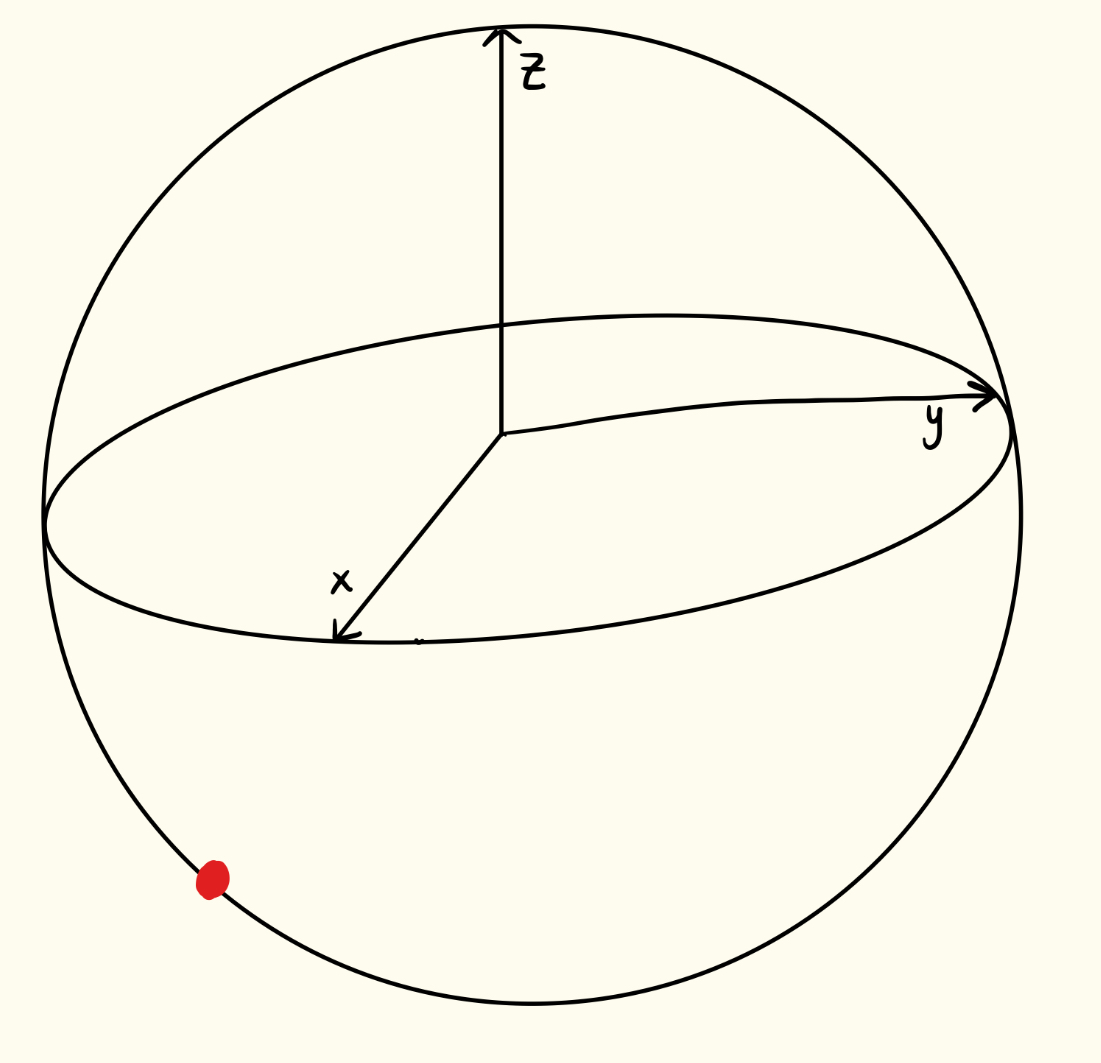
\includegraphics[width=0.3\textwidth]{case_one.jpeg}
        \end{center}
    \end{itemize}
    \item When the control qubit is $|1\rangle$:
    \begin{itemize}
        \item The operator applies $|1\rangle \langle 1| \otimes R_X (\gamma)$
        \item The second qubit undergoes a rotation around the X-axis by angle $\gamma$
        \item Target qubit rotates around the X-axis by angle $\gamma$
        \begin{center}
            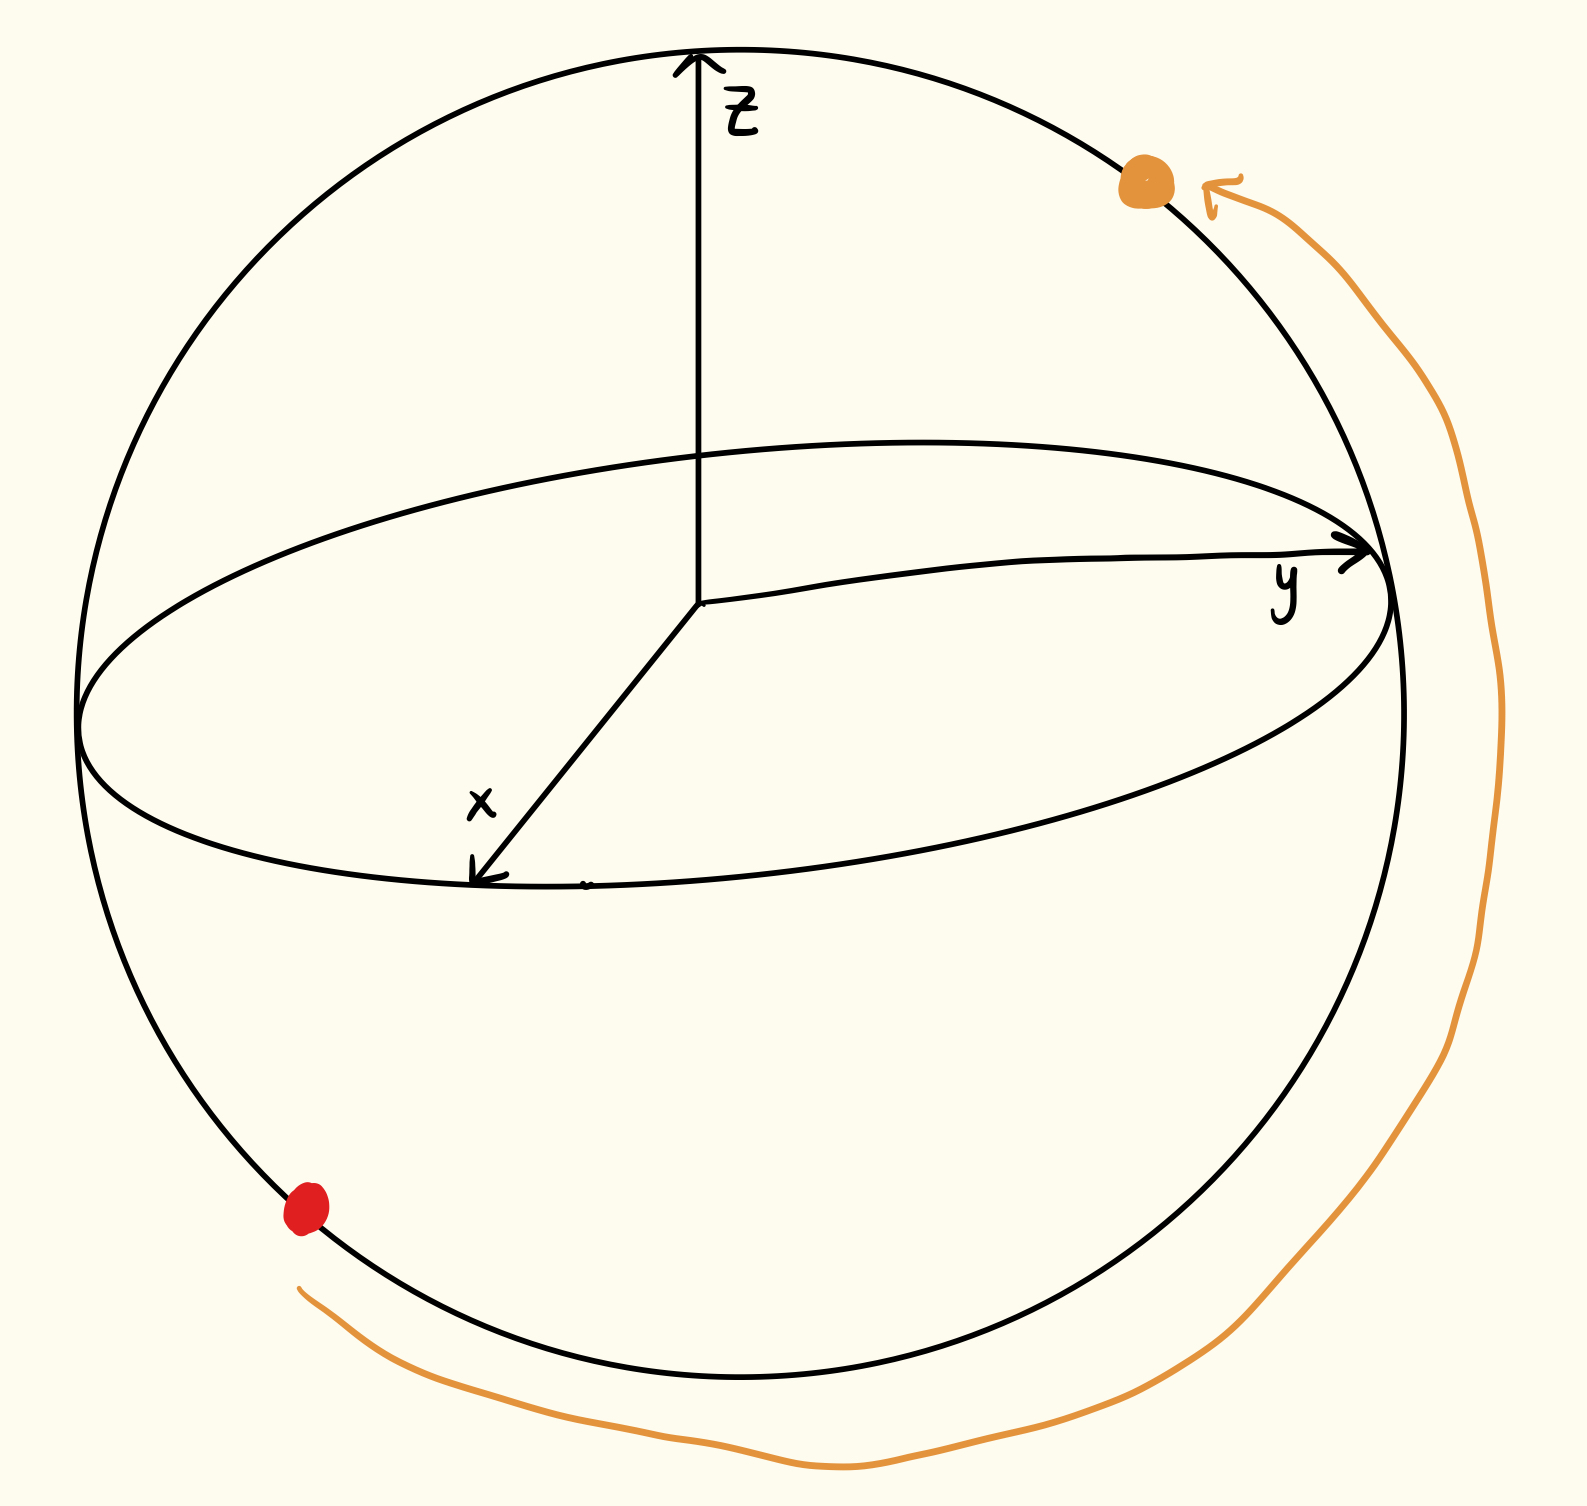
\includegraphics[width=0.3\textwidth]{case_two.jpeg}
        \end{center}
        \item The rotation looks like this becuase it is along the X-axis and since $\gamma \neq \pi$, it will not be a full 180-degree rotation
        \item Therefore, I have represented a 90-degree rotation along the X-axis which would be represented as $R_X (\frac{\pi}{2}) \text{Where, } \gamma = \frac{\pi}{2}$
    \end{itemize}
\end{enumerate}

%%%%%%%%%%%%%%%%%%%%%%%%%%%%%%%%%%%%%%%%%%%%%%%%%%%%%%%%%%%%%%%%%%%

\end{document}